	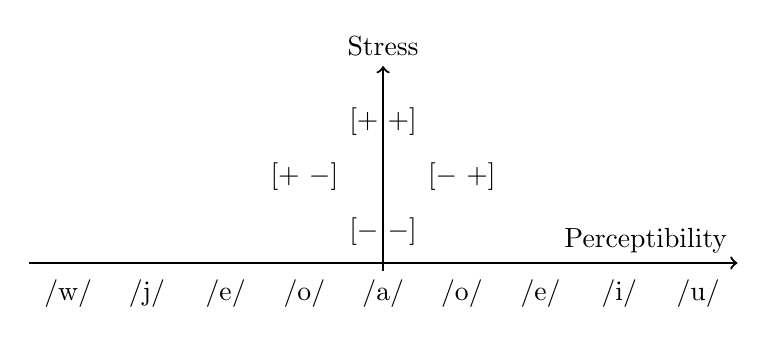
\begin{tikzpicture}
		\def\h{0.68}
		
		\def\tick#1#2#3{\draw[thick,#2] (#1+.09) --++ (0,-.18) node[below=-2pt] {\strut #3};}
		

		%\fill[left color=myred, right color=myyellow] (5,0) rectangle (35,\h);
		%\fill[left color=myyellow,right color=mygreen] (35,0) rectangle (50,\h);
		%\fill[left color=mygreen,right color=myyellow] (50,0) rectangle (65,\h);
		%\fill[left color=myyellow,right color=myred] (65,0) rectangle (95,\h);

		\draw[->,thick] (0,-.1) -- (0,2.5) node[above] {Stress};

		\node[above ] at (0,.1) {[$- \ -$]};
		\node[above] at (-1,.8) {[$+\ -$]};
		\node[above] at (1,.8) {[$-\ +$]};
		\node[above] at (0,1.5) {[$+\ +$]};
	
		
		% INTENSITY
		\draw[->,thick] (-4.5,0) -- (4.5,0) node[above left] {Perceptibility};
		%\draw[->,thick] (20,0) -- (15,0) node[below right=-3,scale=1.1] {};

		%\node[below=-4,scale=0.9] at (15,-3.5) {\strut {$+$}};
		%\node[below=-4,scale=0.9] at (46,-.1) {\strut {$-$}};
		%\node[below=-4,scale=0.9] at (46,1.4) {\strut {$+$}};
		%\node[below=-4,scale=0.9] at (84,-3.5) {\strut {$+$}};
		\node[below=-4] at ( -4,-0.2) {\strut {/w/}};
		\node[below=-4] at ( -3,-0.2) {\strut {/j/}};
		\node[below=-4] at ( -2,-0.2) {\strut /\textsubarch{e}/};
		\node[below=-4] at ( -1,-0.2) {\strut /\textsubarch{o}/};
		\node[below=-4] at ( 0,-0.2) {\strut {/a/}};
		\node[below=-4] at ( 1,-0.2) {\strut /\textsubarch{o}/};
		\node[below=-4] at ( 2,-0.2) {\strut /\textsubarch{e}/};
		\node[below=-4] at ( 3,-0.2) {\strut /\textsubarch{i}/};
		\node[below=-4] at ( 4,-0.2) {\strut /\textsubarch{u}/};

	\end{tikzpicture}
